\graphicspath{{img/results}{img/results/out}}

\chapter{Results}
\label{ch:results}
This chapter will present the results of the smarticle experiments in the TASEP. We will start by setting a baseline with the classical TASEP and analyze how different speed distributions affect this purely stochastic system. Next, we will compare the results with a simple hard-coded policy, before moving on to the smarticle training. We will analyze the results of the smarticle training for different reward structures and compare them to the baseline. 

\section{Notes on measuring time and current}
\label{sec:time_current}
The classical TASEP is defined for continuous time. Each particle moves according to its own internal clock. In the numerical version treated in this thesis, time has to be discretized. The discrete time step should be defined in a way that allows time averages of observables in the discrete version and the continuous version to coincide. We base our time step definition on the fact that in the continuous version, the \textit{average} number of jump attempts per second is constant. We therefore define our time step as a fixed number of \textit{update attempts}. An update attempt is the picking of a random grid cell and the attempt to move the particle in that cell, \textit{if it is occupied}. This means that also in the discrete version, the number of \textit{jump attempts} per second is constant in the time average, while it can fluctuate over short time scales.
\\
\\
In this thesis, the time step is specifically defined as \textit{one} update attempt. This makes it easy to define a particle \textit{current}, which is independent of the system size. The current is defined as the number of actual forward jumps per \textit{update attempt}. This of course has the dimension of a particle current \textit{density}, but it is still called \textit{current} in the lattice gas literature. It is the more useful quantity to work with, as it makes it easy to compare different systems. 
\\
\\
Note that this definition of the time step differs from the prevalent definition of the Monte Carlo time step in the literature \cite[ch. 3.2]{daquila_monte_nodate}, where one time step is defined more naturally as one Monte Carlo sweep. A Monte Carlo sweep is defined as $N$ update attempts, where $N$ is the number of particles in the system. 

\newpage

\section{Setting a Baseline: Classical TASEP}
\label{sec:baseline}
\begin{wrapfigure}{R}{0.45\textwidth}
    \raisebox{0pt}[\dimexpr\height-0.6\baselineskip\relax]{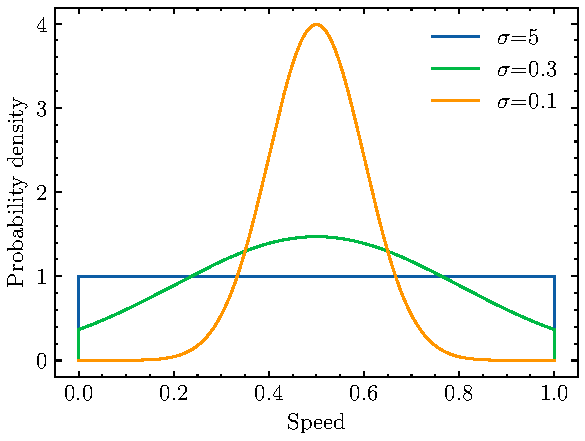
\includegraphics{truncated_normal.pdf}}
    \caption{Normalized truncated normal distributions with mean $\mu=0.5$ and different standard deviations $\sigma$.}
    \label{fig:speed_dists}
\end{wrapfigure}
This section will use the classical 2D (T)ASEP as introduced in section \ref{sec:2d-tasep}. We will make it totally asymmetric in the horizontal direction (the \textit{forward} direction) by setting the probability $p$ to jump forward to $1/2$ and the probability $q$ to jump backward to $0$. The vertical direction (the \textit{up/down} direction) will be symmetric with probabilities $a=b=1/4$. The system has periodic boundary conditions in both directions. We will analyze a $128 \times 32$ system and a narrower $128 \times 6$ system. Both systems will be initialized with a checkerboard pattern of particles and holes, yielding a density of $\rho = 1/2$. This density will be chosen for most experiments, as it is dense enough for the different policies and speed distributions to have a significant effect on the system, but not so dense that the system is always jammed. Speeds will be drawn from a truncated normal distribution with mean $0.5$ and different standard deviations $\sigma$. The distribution is truncated at $0$ and $1$, so that speeds are always in that range. Two example speed distributions are shown in figure \ref{fig:speed_dists}. 

\subsection{Finding the Steady State}

When we want to compare the average current of different ASEP configurations, we have to make sure that the system has reached a steady state. The steady state has been reached when the current fluctuates around a constant mean value without an overall upwards or downwards trend. The time it takes to reach the steady state depends on the system size, the density and the initial conditions. When using a checkerboard setup for example, it's intuitive that the current will be very high in the beginning of the simulation, as every particle has an empty site in front of it and can move forward. As time passes, the probability of being able to move forward decreases (for different reasons that we will examine in the next paragraphs), and the mean current drops, asymptotically approaching the steady state current.
\\
\\
Figures \ref{fig:currents_fixed_sigma_128x32} and \ref{fig:currents_fixed_sigma_128x3} show the current as a function of time steps since initialization of the system to the checkerboard pattern for different speed distribution standard deviations $\sigma$. We can see that for small $\sigma$, when all particles have similar speeds, the current converges quickly and reaches a steady state after about 100,000-150,000 time steps. For larger $\sigma$, particles have different speeds and the equilibration phase takes longer, as jams form and dissolve and slow particles move very rarely. For $\sigma = 5$, especially in the narrow system (Fig. \ref{fig:currents_fixed_sigma_128x3}), we see that the steady state is still not quite reached after 300,000 time steps. 
\\
\\
One could expect the equilibration time to be roughly proportional to the number of Monte Carlo sweeps that have passed. This however is not the case, as we can see by comparing figures \ref{fig:currents_fixed_sigma_128x32} and \ref{fig:currents_fixed_sigma_128x3}. The narrow system has almost 11 times fewer particles than the wide system and thus performs about 11 times more Monte Carlo sweeps in the same number of time steps. However, the equilibration time is not 11 times shorter, but seems to be about the same, or even longer. We can conclude that the number of time steps is a better measure of the equilibration time than the number of Monte Carlo sweeps.
\\
\\
For the following experiments, the steady state current will be calculated by running the simulation for 600,000 time steps and averaging the current over the last 150,000 time steps. This ensures that the system has reached a steady state even for the configurations that take longer to equilibrate.
\\
\begin{figure}[H]
    \centering
    \begin{subfigure}{\textwidth}
        \centering
        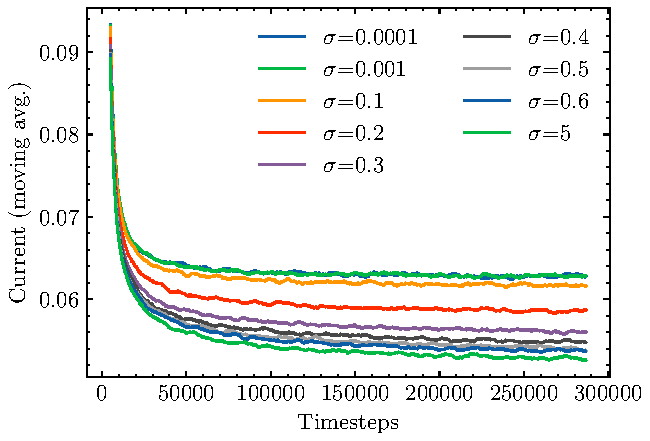
\includegraphics{currents_fixed_sigma_128x32}
        \caption{System size: 128x32}
        \label{fig:currents_fixed_sigma_128x32}
    \end{subfigure}
    \par\vspace{1cm}
    \begin{subfigure}{\textwidth}
        \centering
        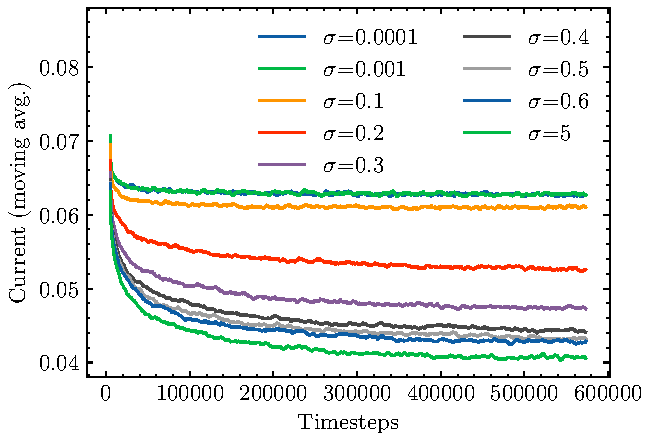
\includegraphics{currents_fixed_sigma_128x3}
        \caption{System size: 128x3}
        \label{fig:currents_fixed_sigma_128x3}
    \end{subfigure}
    \caption{Current as a function of time steps since initialization of the system to the checkerboard pattern for different speed distribution standard deviations $\sigma$ and two different system sizes. The data is averaged over 800 independent runs and plotted with a moving average over 5000 time steps.}
\end{figure}


\section{Steady State Current as a Function of System Size and Speed Distribution}
\label{sec:steady_state_current}
Now that we have established a definition of what is to be measured and how this measurement can be done from the simulation data, we can check if the measured steady state current is in accord with our intuition and how it depends on the system parameters. 

\subsection{Theoretical Expectation}
\label{sec:theoretical_expectations}
In order to derive an expression for the expected value of the current, we closely examine what happens during one time step. This will help us to understand the probability of an actual forward move happening during one time step, which, by our definition, is the current.
\\
The following steps are performed during one time step:
\begin{enumerate}
    \item Pick a random grid cell.
    \item If the cell is occupied (probability $p_{occ}=\rho=0.5$), perform a move attempt as follows:
    \item Check the speed: The move attempt is continued with probability $p_{spd}=\text{speed}$.
    \item If the move attempt is continued, pick a direction (forward has probability $p=1/2$).
    \item If the target cell is empty (probability $p_{emp}\approx 1-\rho$), perform the move.
\end{enumerate}
Where the expression $p_{emp}\approx 1-\rho$ only holds for an approximately uniform density distribution throughout the system. The average speed $\bar{v} = /bar{p_{spd}}$ is the expectation value $\mu$ of the speed distribution, which is set to $0.5$ in all experiments. The total probability of a forward move in one time step is the product of the probabilities of the individual steps:
\begin{align}
    \langle J\rangle &\coloneqq p_{occ} \cdot p_{spd} \cdot p \cdot p_{emp} \label{eq:current_theory} \\
                     &\approx p \cdot \mu \cdot \rho (1-\rho) = \left(\frac{1}{2}\right)^4 \nonumber \\
                     &= 0.0625 \text{.}\nonumber
\end{align}
More thorough derivations of this expression for ASEP systems with equal speeds can be found in the literature, for example in \cite[section 2.3.2]{daquila_monte_nodate}. Equation \ref{eq:current_theory} also confirms that our choice of the density $\rho=1/2$ is optimal for maximizing the current in the system, as the maximum of the function $f(\rho) = \rho(1-\rho)$ is at $\rho=1/2$.


\subsection{Results of the Simulation}
\label{sec:results_simulation_current_sigma_size}
Figure \ref{fig:steady_state_current_sizes_log} shows the steady state current as a function of the speed distribution's standard deviation $\sigma$ for different system sizes. The steady state current has been obtained as explained previously and the data is averaged over 800 independent runs. For all system sizes, we observe a constant maximum current for $\sigma \ll 1$ that is only very slightly above the expected value of $0.0625$. The slight increase is probably due to the fact that the steady state is only reached in the limit of infinite time. Although being very close, after 450,000 time steps, the current is still dropping a tiny amount, as can be seen in figure \ref{fig:currents_fixed_sigma_128x3}. 
\\
As the width of the speed distribution grows to values of $\sigma \approx 1$, the current drops quickly before asymptotically converging to the minimum value, following a horizontally inverted logistic function. The logistic curve's midpoint is at $\sigma_0 \approx 0.2$ and the width of the transition is $\Delta \sigma \approx 1$. This makes sense, as the speed distribution is truncated at $0$ and $1$, so for values of $\sigma$ close to $0$, all particles have speeds close to $0.5$ and the current is close to its maximum value. When $\sigma$ grows, the speeds in the system get more and more diverse, until $\sigma$ reaches $1$, where the speed distribution is almost uniform and doesn't change much anymore. 
\\
The current drops although the mean speed in the system is still the same, because the probability of a particle moving forward is not only dependent on its own speed, but also indirectly on the speeds of the particles in front of it. The slow particles bottleneck the current as the fast particles have to wait for them to move forward, creating a jam. This effect is more pronounced in narrower systems, as small jams block a higher proportion of the system. In wide systems, particles can avoid jams by moving around them, and even if there's a jam in almost every lane, the probability of these jams to all be in the same column is very low. In narrow systems, this can happen, forming a wall of slow particles, which is hard to penetrate. This is clearly visible in figure \ref{fig:steady_state_current_sizes_log}, where the total drop in current is much higher for narrow systems. 
\\
\\
Looking back at equation \ref{eq:current_theory}, we can also try to explain this behavior theoretically. When jams form, the density in the system is not uniform anymore. Instead, there are regions of high density (jams) and regions of low density (empty lanes). This increases the mean density in the neighborhood of a random particle, decreasing $p_{emp}=(1-\rho)$ and thus the probability of a forward move.  

\begin{figure}[H]
    \centering
    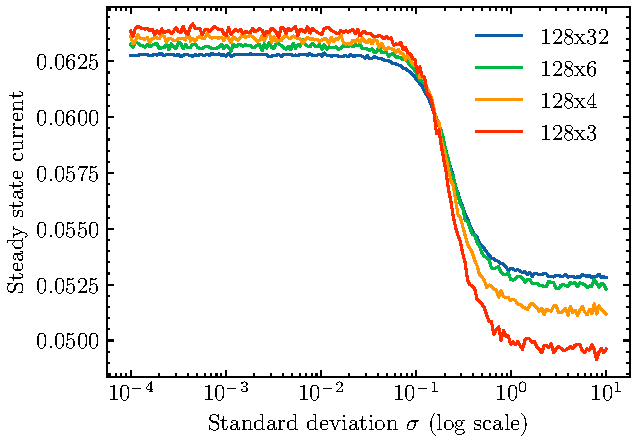
\includegraphics{steady_state_current_sizes_log.pdf}
    \caption{Steady state current as a function of the speed distribution's standard deviation $\sigma$ for different system sizes. Steady state current is calculated as the average current over all remaining time steps after the steady state has been reached (the current has stopped dropping). The data is averaged over 800 independent runs.}
    \label{fig:steady_state_current_sizes_log}
\end{figure}

\section{A Naive Policy}
We have now established a baseline current for different system sizes and speed distributions. Before we move on to the smarticle training to try to optimize the current with reinforcement learning, let's see if we can improve the current with a simple hard-coded policy. 
\\
One of the simplest and yet effective policies is to always move forward if possible. Especially when we choose $\sigma$ to be very small and all particles have similar speeds, this policy should be very effective, as it keeps the density uniform and avoids jams. Furthermore, it is very easy to implement without writing any new code by just setting the probability $p$ to move forward to $1$ and all other probabilities ($a,b,q$) to $0$.
\\
\\
Figure \ref{fig:steady_state_current_always_forward} compares the steady state current of this policy with the current from the last experiment, again as a function of the width of the truncated normal distribution. We can see that for small $\sigma$, our policy drastically improves the current, approximately doubling it. For larger $\sigma$, the current drops as before and drops even further, resulting in only about half the current of the baseline for $\sigma\gg 1$. 
\\
\\
The reason for the extreme drop in current is that the policy is not able to deal with jams at all. The current in each lane is limited to the speed of the slowest particle in that lane. The resulting measured current then is the average of the currents in all lanes. 
\\
\begin{figure}[H]
    \centering
    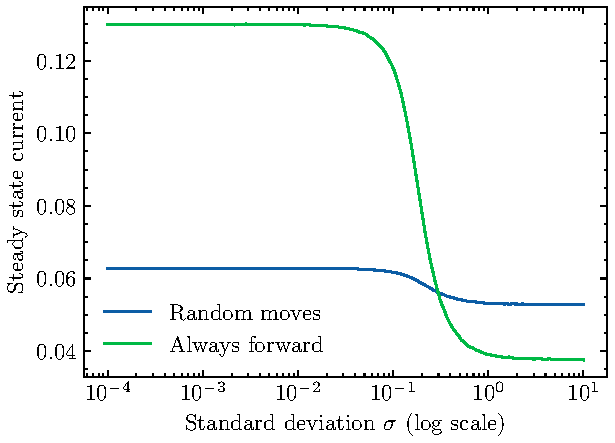
\includegraphics{steady_state_current_both_log.pdf}
    \caption{Steady state current as a function of the speed distribution's standard deviation $\sigma$ for two different ASEP configurations. \enquote{Random moves} has a probability of $p=1/2$ to move forward probabilities $a=b=1/4$ to move up/down. \enquote{Always forward} has $p=1$ and $a=b=0$. A system of size 128x32 was used. The data is averaged over 800 independent runs.}
    \label{fig:steady_state_current_always_forward}
\end{figure}
The current achieved by this policy for small $\sigma$ is even more interesting. It can be used as a new, very strong baseline for the smarticle training in systems with equal speeds. At first glance, it might even seem like the theoretical maximum current. Finding this maximum analytically is not trivial and goes beyond the scope of this thesis. However, we can try to find an upper bound for the current by looking at equation \ref{eq:current_theory} again:
\begin{align*}
    \max(\langle J\rangle) &= \max(p_{occ} \cdot p_{spd} \cdot p \cdot p_{emp}) \\
                           &\le \max(p_{occ}) \cdot \max(p_{spd}) \cdot \max(p) \cdot \max(p_{emp}) \\
                           &= \rho \cdot \mu \cdot 1 \cdot \max(p_{emp}) \\
                            &= 0.25 \cdot \max(p_{emp})\text{,}
\end{align*}
where $\max(x)$ is the maximum expected value of $x$ at a random time step, for a randomly picked particle. It therefore represents the maximum time-averaged value of $x$ that can be achieved by any policy. I have set $p_{occ}=\rho$, $p_{spd}=\mu$, as they are external parameters that cannot be optimized by a policy. The policy cannot influence which particle is picked at a given time step, so it cannot influence $p_{occ}$. The \textit{average} speed of a random particle will also always be the mean speed $\mu$. The maximum of $p$ that any policy can have is obviously $1$ (in general, this will not be a probability when using a policy, but the decision will be based on the particle's observation, but the maximum fraction of forward decisions is still 1). 
\\
The last factor, $max(p_{emp})$, is the hardest to approximate. There are configurations where $p_{emp}$ reaches its maximum value of $1$, but these configurations cannot last longer than one time step. In the checkerboard configuration for example, every particle has an empty site in front of it, so $p_{emp}=1$. However, as soon as one particle moves forward, two particles are immediately next to each other and $p_{emp}$ decreases. We therefore know that $\max(p_{emp})<1$.
\\
On the other hand, we know that $\max(p_{emp})\ge0.5=(1-\rho)$, as this upper bound is reached by the \enquote{always forward} policy. This places the upper bound for the current at
\begin{equation}
    0.25 > \max(\langle J\rangle) \ge 0.25 \cdot (1-\rho) = 0.125 \text{.}
\end{equation}
In order to keep $p_{emp}$ above $1-\rho$, which it would be for a randomized configuration, a policy has to intelligently fight against the disorder inevitably introduced by the random picking of particles. This is especially hard for systems with equal speeds, as the density in these systems has to be kept uniform, while also moving forward as often as possible.
\\
In the regime of high $\sigma$, where the \enquote{always forward} policy performs very poorly, $p_{emp}$ becomes a very interesting point of attack for a current-optimizing policy. When particles have very different speeds, a policy can organize the system in a way that slow particles are more densely packed than fast particles, increasing $p_{emp}$ for the fast particles while decreasing it for the slow particles. This increases the net current, as the fast particles can fulfill their potential to move forward more often. We will investigate this in more detail in the next sections.


\section{Smarticles for Current Optimization}
\label{sec:smarticle_current_optimization}
This section will present the results of different smarticle trainings for slightly different goals. The main goal is always to maximize the current, but we will different approaches to achieve this goal, utilizing many of the features of the python package introduced in section \ref{sec:implementation-smarttasep}. Although the deep Q-learning algorithm is not deterministic e.g. due to the random initialization of the neural network weights, the results presented here have shown to be reproducible. Appendix \ref{app:code} contains the code that is needed to reproduce the results with the smart TASEP python package.

\subsection{First Training: Equal Speeds}
As a first experiment, we will try to maximize the current in a system with equal speeds. We will use a system of size $128 \times 24$ and a speed distribution with $\sigma=10^-4$. The reward structure for this first experiment is very simple and includes only the \texttt{social\_reward} in addition to the default reward. Optimal hyperparameters for this reward structure have already been found in section \ref{sec:hyperparam_optim}. The training was run for 500,000 time steps, with a reset of the environment after every 100,000 time steps.
\\
Figure \ref{fig:first_training_screenshot} shows a screenshot of the real-time visualization of the training after $\approx 350,000$ time steps. We can see that the training is almost converged at this point, confirming that $500,000$ time steps is enough to reach convergence for this problem. After the training, the simulation was run with a greedy policy for another $1.5$ million time steps to measure the steady state current. The results are shown in figure 

\begin{figure}
    \centering
    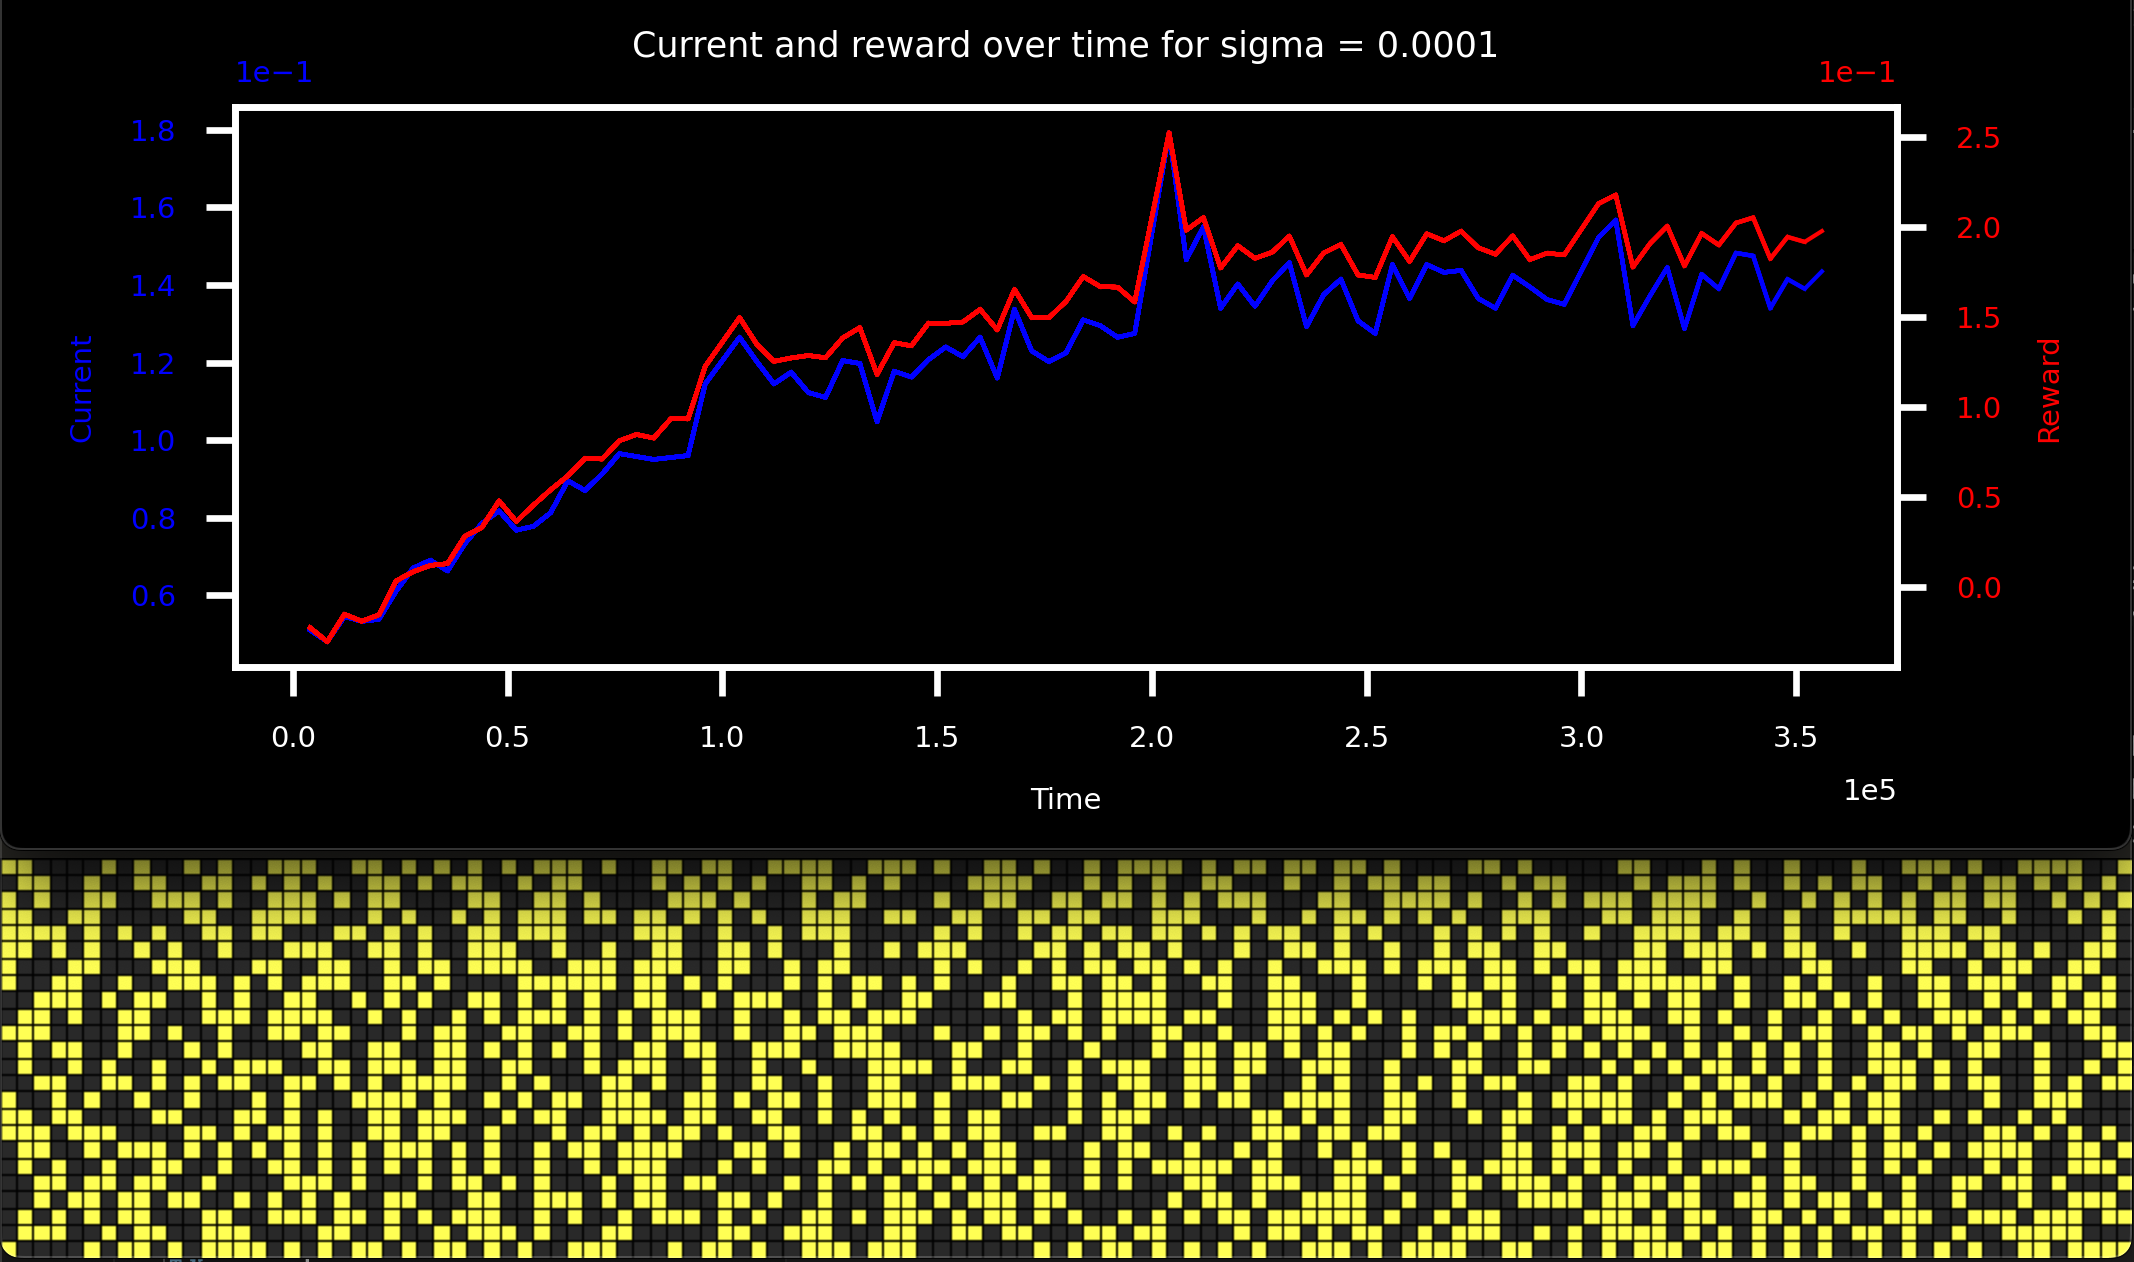
\includegraphics[width=\textwidth]{first_training_screenshot.png}
    \caption{A screenshot of the real-time visualization of the first training, taken after $\approx 350,000$ time steps. All particles have the same speed of $0.5$, which can also be seen from their yellow color. We can see that the algorithm has almost converged at this point.}
    \label{fig:first_training_screenshot}
\end{figure}

\begin{figure}
    \centering
    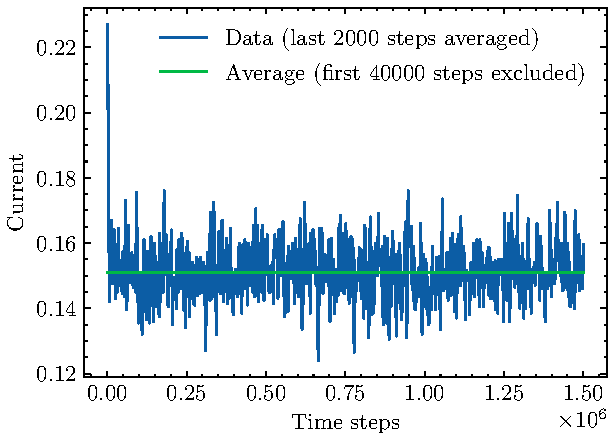
\includegraphics{equal_speeds.pdf}
    \caption{Steady state current as a function of the simulation time for the first trained smarticle agent. The green line shows the average current, which is at about $0.152$, outperforming not just the baseline by about 143\%, but also the \enquote{always forward} policy by about 22\%.}
\end{figure}